\documentclass{article}
\usepackage{tikz}
\usetikzlibrary{patterns}

\begin{document}

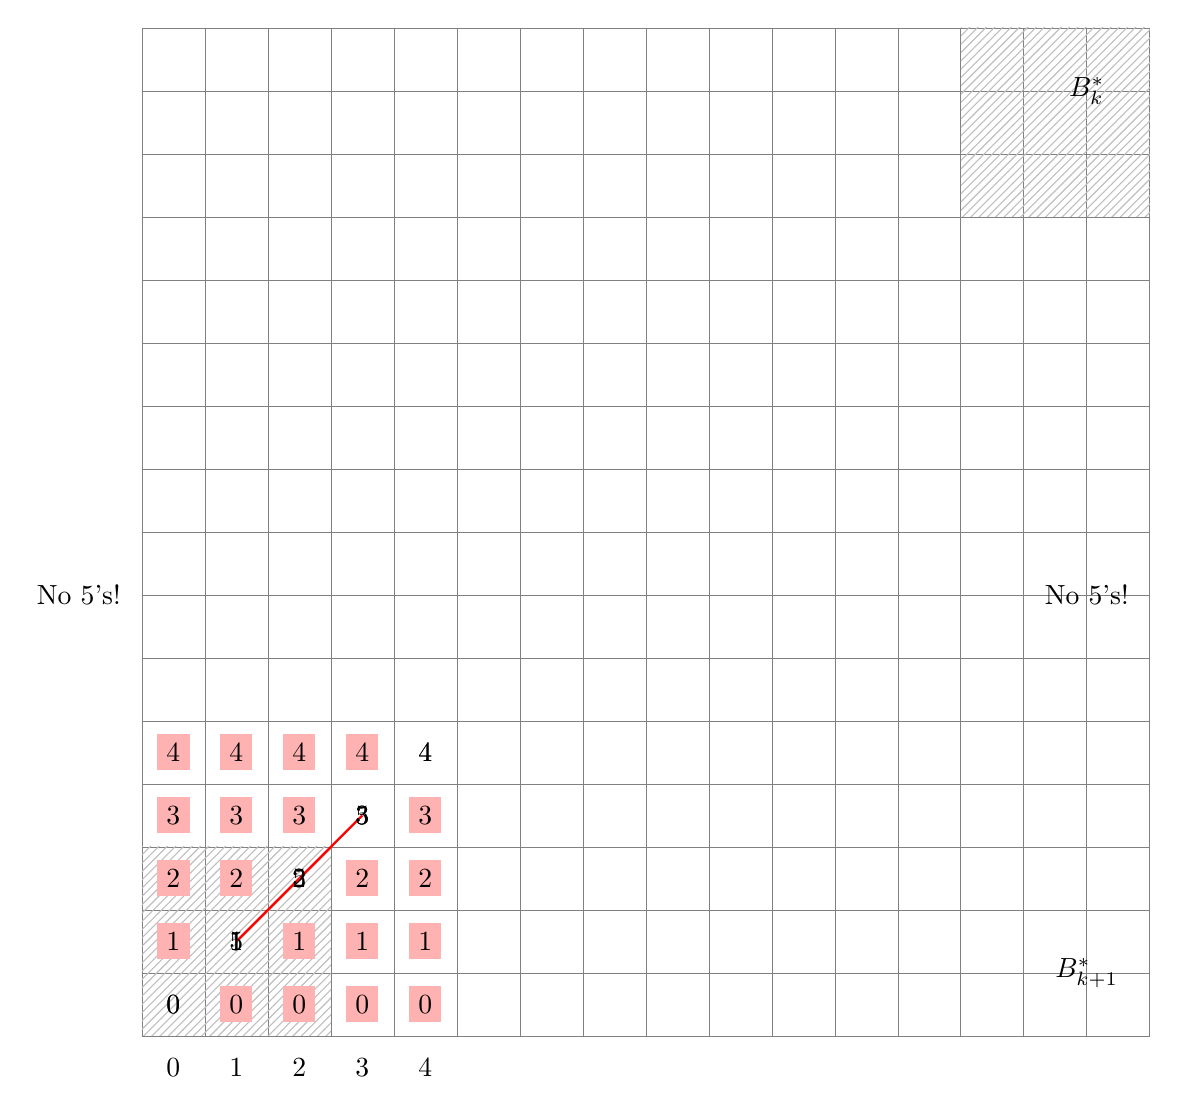
\begin{tikzpicture}[scale=0.8]
    % Draw the grid
    \draw[help lines] (0,0) grid (16,16);
    
    % Draw the shaded regions
    \fill[pattern=north east lines, pattern color=gray!50] (0,0) rectangle (3,3);
    \fill[pattern=north east lines, pattern color=gray!50] (13,13) rectangle (16,16);
    
    % Draw the numbers
    \foreach \x in {0,...,4} {
        \node at (\x+.5,-.5) {\x};
        \foreach \y in {0,...,4} {
            \node at (\x+.5,\y+.5) {\y};
        }
    }
    
    % Draw the red segments indicating shadowed areas
    \draw[red, thick] (1.5,1.5) -- (2.5,2.5);
    \draw[red, thick] (2.5,2.5) -- (3.5,3.5);
    
    % Draw the labels
    \node at (-1,7) {No 5's!};
    \node at (15,7) {No 5's!};
    \node at (15,15) {$B_k^*$};
    \node at (15,1) {$B_{k+1}^*$};
    
    % Draw the numbers in the shadowed regions
    \node at (1.5,1.5) {5};
    \node at (2.5,2.5) {5};
    \node at (3.5,3.5) {5};
    
    % Draw the numbers in the light red cells
    \foreach \x in {0,...,4} {
        \foreach \y in {0,...,4} {
            \ifnum\x=\y
                \node at (\x+.5,\y+.5) {\y};
            \else
                \node[fill=red!30] at (\x+.5,\y+.5) {\y};
            \fi
        }
    }
\end{tikzpicture}

\end{document}